\documentclass[12pt,a4paper]{scrartcl}
\usepackage[utf8]{inputenc}
%\usepackage[latin1]{inputenc} %  Alternativ unter Windows
\usepackage[T1]{fontenc}
\usepackage[paper=a4paper,
	left=25mm,
	right=25mm,
	top=25mm,
	bottom=20mm]{geometry}
\usepackage[nottoc]{tocbibind}
\usepackage[ngerman]{babel}
\usepackage[pdftex]{graphicx}
\usepackage{latexsym}
\usepackage{amsmath,amssymb,amsthm,amsfonts}
\usepackage{mathtools}
\usepackage{enumitem}
\usepackage[utf8]{inputenc}
\usepackage{float}
\usepackage{subfigure}
\newcommand{\R}{\mathbb{R}}

\DeclareMathOperator{\dive}{div}
\newtheorem{Satz}{Satz}[section]\newtheorem{Definition}[Satz]{Definition} 
\newtheorem{Lemma}{Lemma}		                 
\newtheorem{Korollar}[Satz]{Korollar}
\newtheorem{Proposition}[Satz]{Proposition}                  
\newtheorem{examples}[Satz]{Beispiel}
\let\oldexamples\examples
\renewcommand{\examples}{\oldexamples\normalfont}
\newtheorem*{notation}{Notation}
\let\oldnotation\notation
\renewcommand{\notation}{\oldnotation\normalfont}
\newtheorem*{remark}{Bemerkung}
\let\oldremark\remark
\renewcommand{\remark}{\oldremark\normalfont}                  


\usepackage{csquotes}[german = quotes]
\usepackage{xcolor}
\newcommand*\diff{\mathop{}\!\mathrm{d}}
\DeclareMathOperator{\conv}{conv}
\DeclareMathOperator{\spann}{span}
\DeclareMathOperator{\Jacobi}{D}
\DeclareMathOperator{\diam}{diam}
\definecolor{Mygreen}{RGB}{0,128,0}
\newcommand{\defi}[1]{\textcolor{Mygreen}{#1}}
\renewcommand{\phi}{\varphi}
\renewcommand{\epsilon}{\varepsilon}
                              
\numberwithin{equation}{section} 

% Praktikumsbericht nummer setzen
\newcommand{\BerichtNR}{1}

\begin{document}
\begin{titlepage}
	
\includegraphics[scale=0.5]{kit-logo.jpg} 
	\begin{center} 
		\LARGE 
		\vspace*{2cm}
		\LARGE Praktikumsbericht \BerichtNR
		\vspace*{1.0cm}
		\hrule
		\vspace*{0.2cm}
		{\vspace{0.2cm} \huge Einführung in das Wissenschaftliche Rechnen}\vspace{0.5cm}
		\hrule
		\vspace*{2.5cm}
		\Large Stefan Karch \\
		Florian Döttling \\
		Tim Buchholz  \\
		\vspace*{1cm}
		20.05.2019 \\
		\vspace*{1.5cm}
		\vspace*{4.0cm}
		\Large Betreuung: Prof. Dr. Christian Wieners, Niklas Baumgarten \\[0.5cm]
		\Large Fakultät für Mathematik \\
		\Large Karlsruher Institut für Technologie
	\end{center}
\end{titlepage}

%\tableofcontents
%\newpage 
%\pagestyle{headings}

\section{Problemstellung}



\subsection{Aufagba blub}
\begin{figure}[H]
	\centering
	\captionabove{Lösungen mit gemischten FEM}
	\subfigure[des Problems 'Simple']{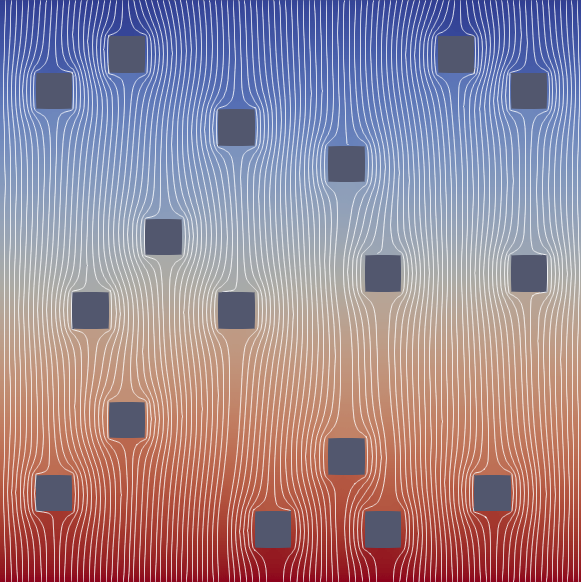
\includegraphics[width=0.49\textwidth]{../14.1.Simple/figrand(1).png}}
	\subfigure[des Problems 'Discontinuous']{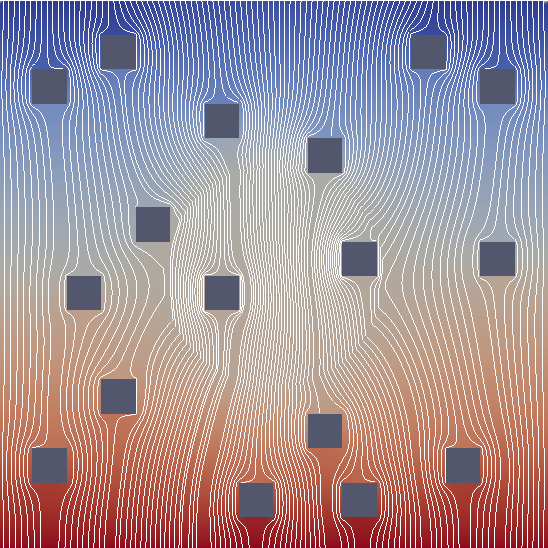
\includegraphics[width=0.49\textwidth]{../14.1.Disc/figrand(1).png}}

\end{figure}

\begin{figure}[H]
	\centering
	\captionabove{Lösungen mit linearen FEM}
	\subfigure[des Problems 'Simple']{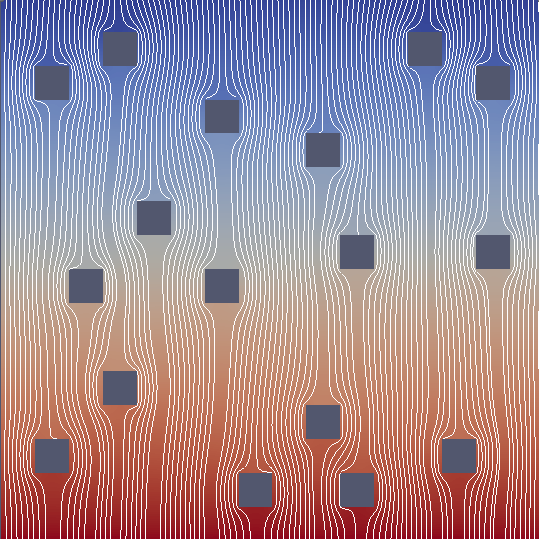
\includegraphics[width=0.49\textwidth]{../14.1.Simple/figrandold.png}}
	\subfigure[des Problems 'Discontinuous']{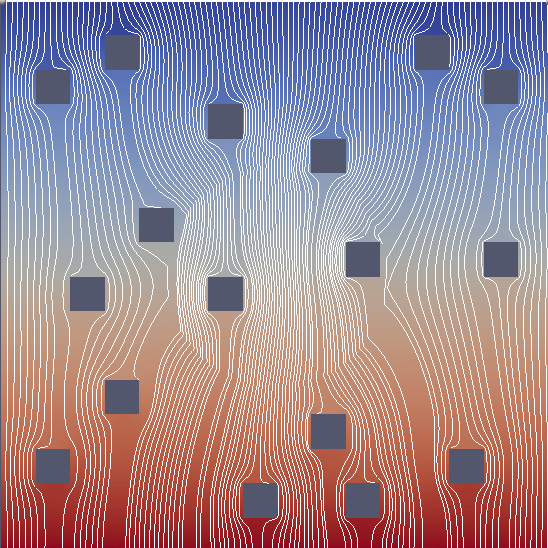
\includegraphics[width=0.49\textwidth]{../14.1.Disc/figrandold.png}}

\end{figure}

Beim Lösen des in der Aufgabe gegebenen Sattelpunktproblems konnte verifiziert werden, dass beim Lösen mit gemischten Finiten Elementen die Ein- und Ausflussbedingung für alle verwendeten Level erhalten werden.
Im Gegensatz dazu stehen die Erkenntnisse, welche wir bereits im letzten Bericht zu den linearen Finiten Elementen gewonnen haben. 
Am deutlichsten spiegelt sich dies in der Größe 'Flux Loss' wieder, welcher bei Verwendung von gemischten Finiten Elementen unabhängig vom Level gleich 0 ist, während er unter Verwendung von linearen Finiten Elementen auf einem komplizierten Mesh nicht zu vernachlässigen ist.  \newline
In den Plots lassen sich bei genauerem Betrachten vor allem im Bereich der Steine des Meshes 'Square500' geringe Unterschiede zwischen beiden Verfahren erkennen. Während die gemischten Finite Elemente sich etwas besser an die Steine 'anschmiegen', lassen sich vor allem die deutlich größeren 'Schatten' unter den Steinen bei den linearen Finiten Elementen erkennen.
Beides lässt sich bei beiden Problemen verifizieren. 

\subsection{Aufgabe 19}
\begin{figure}[H]
	\centering
	\captionabove{Problem Rock}
	\subfigure[Problemstellung]{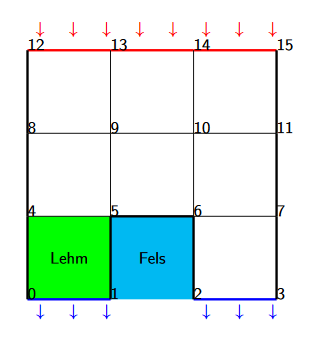
\includegraphics[width=0.4\textwidth]{../problem.png}}
	\subfigure[Definitionen in Rock.geo]{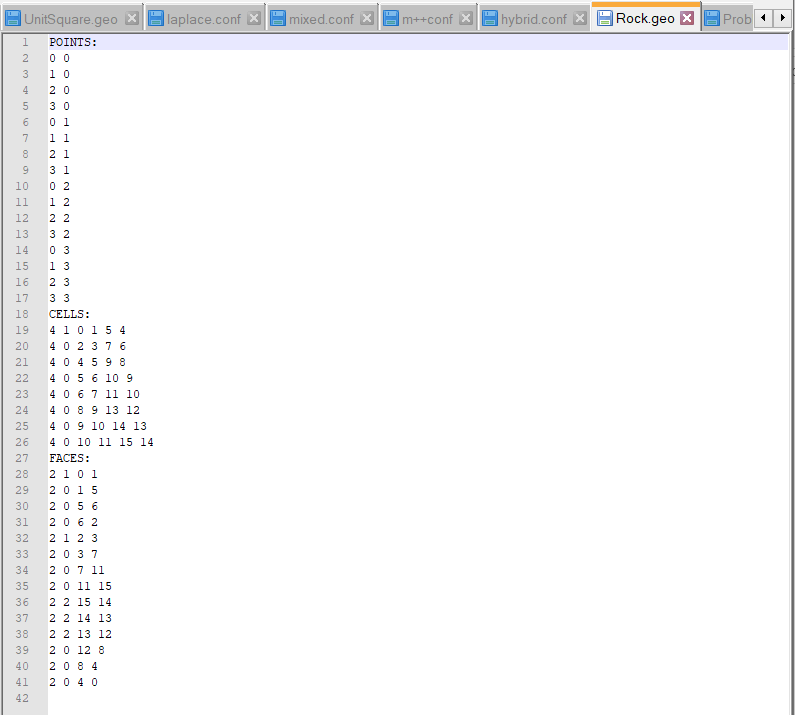
\includegraphics[width=0.59\textwidth]{../rockgeo.png}}
\end{figure}
Ziel der Aufgabe war es das in Abb.3 (a) zu sehende Problem zu implementieren, bzw. vorhandene Lücken in der Implementierung zu schließen.
Zunächst haben wir dafür das Gitter samt Rändern in der Datei Rock.geo definiert. 
Auf eine nähere Erklärung des .geo-Files möchten wir an dieser Stelle verzichten und verweisen auf den ersten Praktikumsbericht.


\begin{figure}[H]
	\centering
	\captionabove{Funktion Permeability der  Klasse RockProblem}
	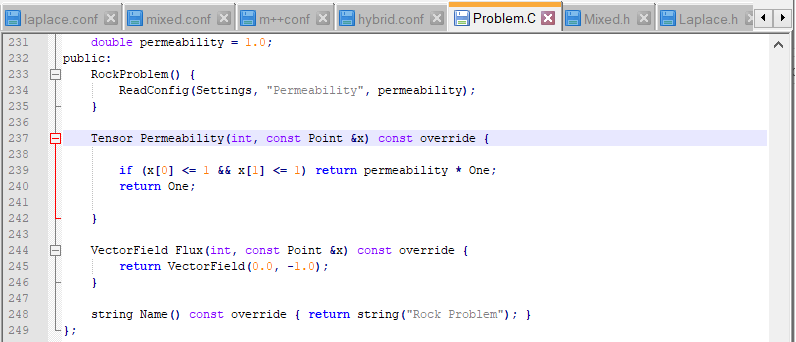
\includegraphics[width=\textwidth]{../permprob.png}	
\end{figure}
In der Datei Problem.C haben wir anschließend die Funktion Permeability der Klasse RockProblem geschrieben.
Ein Punkt (x,y) ist genau dann im unteren linken Kästchen, wenn seine Maximumnorm des zugehörigen Ortsvektors kleiner oder gleich 1 ist. 
Das ist gleichbedeutend mit dem komponentenweisen Vergleich, welchen wir in Zeile 239 durchführen.


\begin{figure}[H]
	\centering
	\captionabove{Funktion OutFlowLeftRight in mixed.h}
	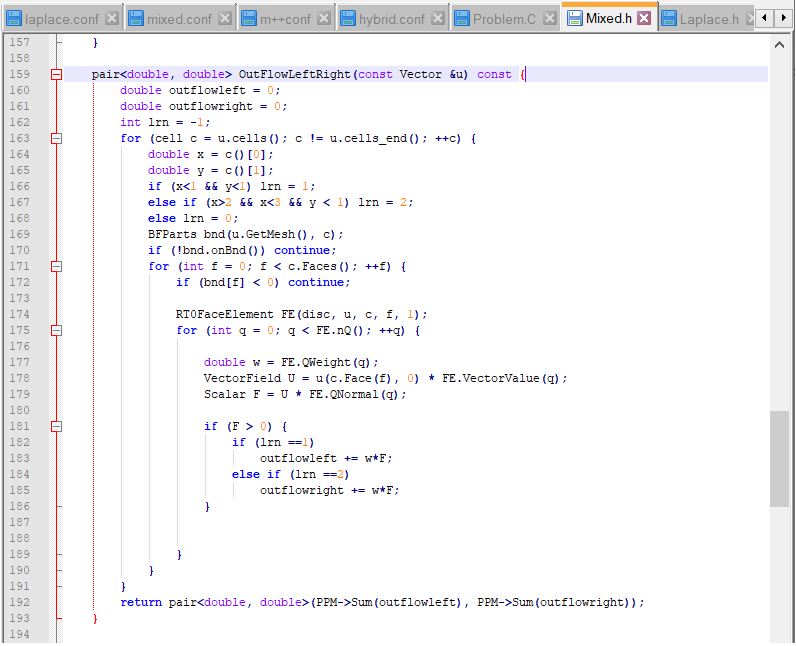
\includegraphics[width=\textwidth]{../mixedoutflow.png}
	
\end{figure}
In der Funktion OutFlowLeftRight

\begin{figure}[H]
	\centering
	\captionabove{Funktion OutFlowLeftRight in Laplace.h}
	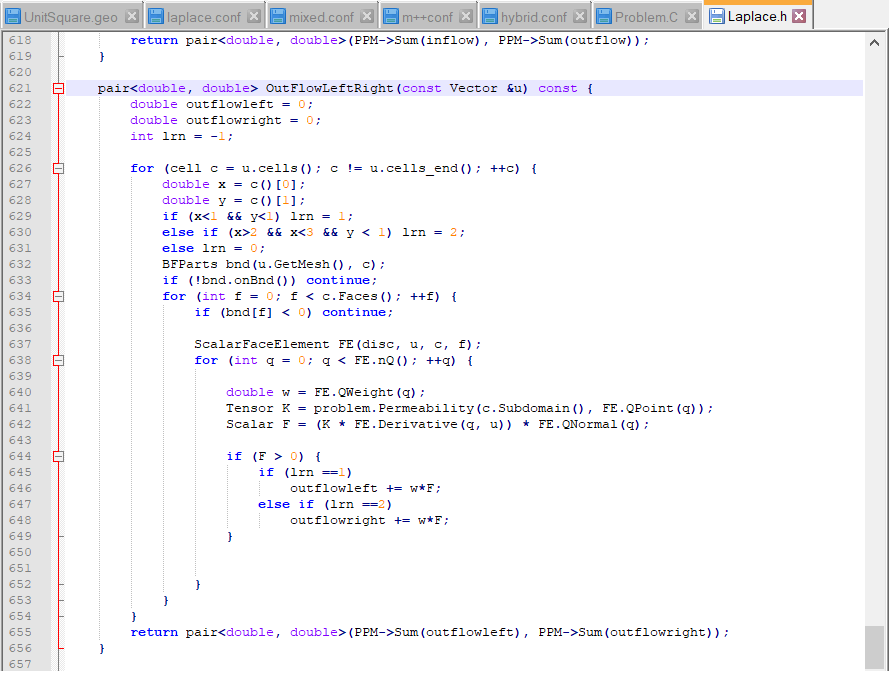
\includegraphics[width=\textwidth]{../laplaceoutflow.png}
	
\end{figure}







\end{document}

